\section[\textit{Random C. V. Generator}]{\textit{Random Control Voltage Generator}}
\sectionmark{\textit{Random C. V. Generator}}
\label{sec:random_generator}

\subsection{La aleatoriedad en el Synthi 100}
Uno de las cualidades que hacen diferentes e interesantes las ejecuciones musicales humanas es el mayor o menor grado de impredicibilidad de sus movimientos, que se traduce en ligeras variaciones aleatorias. De este indeterminismo se ha hecho gala frecuentemente, quizás haciendo de tripas corazón, en los sintetizadores analógicos en general, y en el Synthi 100. Sus circuitos son sensibles a los cambios de humedad y temperatura hasta el punto de que un mismo \textit{patch} y valores de los controles de los diversos módulos puede tener resultados sonoros completamente diferentes en función de las diversas condiciones ambientales en las que se le haga funcionar. 

Pero no todo es aleatoriedad incontrolada. Este módulo (junto al de \textit{Noise Generators} en \ref{sec:noise_generators}), permite <<inyectar>> cierta dosis de aleatoriedad al sistema de forma intencionada. Su disposición de salidas y diales, como se verá más abajo, está inspirado en el funcionamiento de los teclados de la época, que enviaban información ---por voltaje--- de la nota pulsada (frecuencia), velocidad de pulsación (intensidad) y la información de subida y bajada de la tecla (\textit{gate}). De algún modo, este módulo equivale a la ejecución aleatoria de teclas atacadas con diferentes velocidades.


\subsection{Los diales del módulo}
Los dos primeros diales, \textit{Mean} y \textit{Variance} bastan para establecer la frecuencia del cambio de los voltajes de salida. La media temporal entre los cambios es controlada por \textit{Mean}. Los valores reales de tiempo entre cambios serán más próximos a esta media en tanto en cuanto \textit{Variance} sea más cercana a 0, y más dispersos aleatoriamente de esta media cuanto más se aleje de 0. Los tres diales de la derecha tienen como única función  la de controlar la amplitud del voltaje de salida. Aunque el cambio de voltaje se establece al mismo tiempo en \textit{Voltage 1} y \textit{Voltage 2}, el valor de cada uno de ellos es aleatorio y el rango en el que estos valores se mueve es independiente y variado por ambos diales. Por último, \textit{Key}, a modo de <<tecla>> cumple con la función de abrir un \textit{gate} y cerrarlo brevemente cada vez que se produce un cambio en los voltajes.

El hecho de que los cambios sean simultáneos permite eventos sonoros con dos parámetros aleatorios e independientes. Típicamente, es posible crear notas musicales en los que \textit{Voltage 1} controla, pongamos por caso, la frecuencia, mientras que \textit{Voltage 2}, la intensidad. \textit{Key} comunica a una envolvente el inicio y fin de cada nota. Evidentemente, su uso no está reducido a este ejemplo musical, pero su simplicidad permite comprender mejor el funcionamiento de este módulo.

A modo de resumen, estos son los parámetros que se nos permite modificar:

\begin{description}
	\item[\textit{Mean}] Tiempo medio entre cambios de voltaje. 
	\item[\textit{Variance}] Varianza en torno al tiempo medio.
	\item[\textit{Voltage 1}] Voltaje de salida 1.
	\item[\textit{Voltage 2}] Voltaje de salida 2.
	\item[\textit{Key}] A modo de \textit{gate}, esta salida de voltaje tiene un valor distinto de 0 entre cambios, mientras que tiene valor 0 durante un tiempo breve en cada cambio.
\end{description}


\begin{figure}
	\centering
	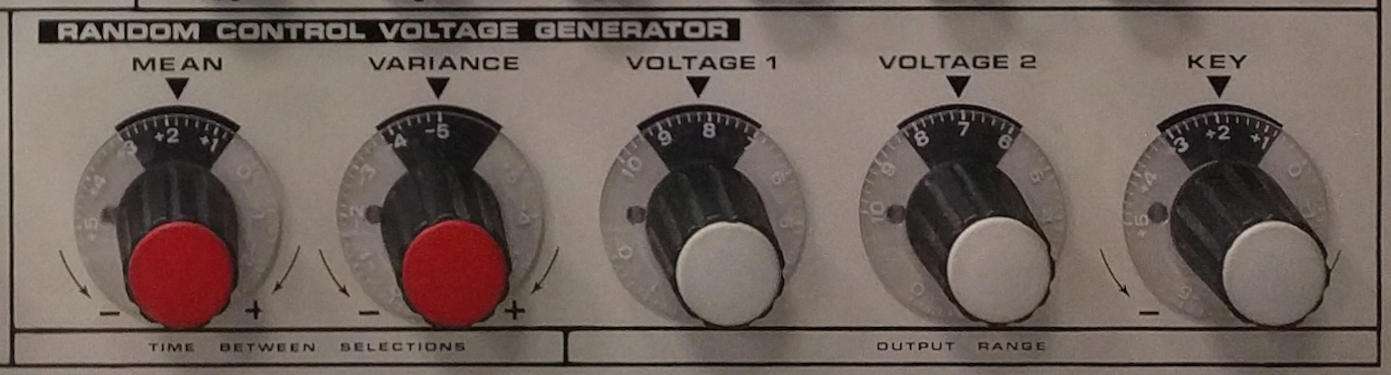
\includegraphics[width=1\textwidth]{images/random_generator}
	\caption[\textit{Random Voltage Control Generator}]{Unidad del generador aleatorio de voltaje de control del Synthi 100 del GME, uno de los pocos módulos que no tiene más que una instancia.}
	\label{fig:random_generator}
\end{figure}

\subsection{Las salidas de voltaje}

Haciendo honor al propio nombre del módulo, las salidas de este son únicamente de voltaje. Las tres salidas coinciden con los tres diales de ganancia, \textit{Voltage 1}, \textit{Voltage 2} y \textit{Key}.


\subsection{Implementación en \appName}
Este es el único módulo cuyo generador de señales no está dirigido por una instancia de \texttt{Synth} sino por un \texttt{Routine}. Un \texttt{Synth} es utilizado únicamente para convertir los valores numéricos del \texttt{Routine} a valores de audio y de control. Una <<rutina>> en SuperCollider puede explicarse como una serie de eventos que se suceden uno tras otro y que pueden ejecutarse asíncronamente. Una característica interesante es la posibilidad de situar en el tiempo estos eventos, haciendo esperar a la rutina un número determinado de segundos con el método \texttt{wait(Integer)}. La rutina que gobierna el módulo \textit{Random Control Voltage Generator} se compone de un bucle de valores aleatorios que se suceden con esperas de duración variable. Los valores aleatorios son generados por métodos del propio lenguaje de programación.

Existen ciertas decisiones arbitrarias tomadas a la hora de crear el código de \appName. Como en todos los módulos, el rango de los valores se ha tomado dentro de unos límites razonables para poder trabajar con él, siempre que no se haya encontrado ninguna indicación técnica en las fichas de los 70 sobre EMS Synthi 100. En \textit{Variance} se ha ignorado el hecho de que su rango en el dial esta comprendido entre $-5$ y 5, haciendo que la varianza sea mayor o menor según su valor también lo es, sin que 0 tenga un significado especial. Esta cuestión ha de ser resuelta empíricamente en el propio GME.